\documentclass{report}
% Packages
\usepackage[utf8]{inputenc}
\usepackage{babel}
\usepackage{amsmath}
\usepackage{amssymb}
\usepackage{amsthm}
\usepackage{graphicx}
\usepackage{float}
\usepackage{listings}
\usepackage{hyperref}
\usepackage[square,sort,comma,numbers]{natbib}
\usepackage{url}
\usepackage{pgfgantt}
\usepackage[strings]{underscore}
\usepackage{booktabs}
\usepackage{geometry}
\usepackage{tabularray} % Required for longtblr

\hypersetup{
    colorlinks=true,
    linkcolor=blue,
    filecolor=magenta,      
    urlcolor=cyan,
    pdftitle={Overleaf Example},
    pdfpagemode=FullScreen,
}

\setlength{\parindent}{0pt} % Remove paragraph indentation

\begin{document}

\begin{titlepage}
    \begin{center}
        \vspace*{1cm}
 
        \Large\textbf{AñadaMaster: K-VATA}
 
        \vspace{0.5cm}
            Memoria trabajo final
        \vspace{1.5cm}
 
        \textbf{Antonio Cabrera, Alejandro Jiménez y Antonio Pérez}
 
        \vfill
             
        Trabajo para el doble grado de\\
        Ingeniería del Software y Matemática Computacional\\
             
        \vspace{0.8cm}
      
        
\includegraphics[width=0.4\textwidth]{figures/logo-u-tad.png}
             
        Ingeniería Software\\
        U-tad\\
        España\\
        Diciembre 2024
             
    \end{center}
 \end{titlepage}

\tableofcontents

\listoffigures

\chapter{Metodología de la empresa}

\section{Investigación previa}

\subsection{Metodologías Ágiles}

\subsubsection{Scrum}

Es una forma de organizar el trabajo en ciclos cortos denominados sprints, estos ciclos suelen durar de entre 2 a 4 semanas, con la idea de aumentar la calidad del producto en cada entrega o añadir funcionalidades nuevas.\\

Dentro de esta metodología existen varios roles importantes Scrum Master (facilita los procesos y elimina obstáculos), Product Owner (gestiona el backlog y prioriza tareas) y Equipo de Desarrollo (Realiza el trabajo técnico).\\

Además, tiene ciertas características que lo distingue, como los distintos tipos de reuniones Daily Scrum (), Sprint Planning (para planificar el próximo ciclo de Sprint) y Sprint Review (tras terminar el sprint).\\

Funciona muy bien en proyectos con requisitos cambiantes.

\subsubsection{Kanban}

Un método visual de gestión de flujo de trabajo que utiliza un tablero Kanban para rastrear las tareas desde “Por Hacer” hasta “Terminado” (como un trello). Este método tiene el objetivo de limitar el trabajo en proceso, evitando la sobrecarga de este, y mejorar continuamente los procesos. Por otro lado, no hacen falta iteraciones fijas. Funciona muy bien en equipos con tareas recurrentes o impredecibles

\subsubsection{Safe}

Una forma de implementar las metodologías ágiles en empresas grandes, consiguiendo una coordinación entre varios equipos. Este método implementa el Scrum o/y el Kanban, ya que une varios equipos ágiles que usan estas metodologías, aplicando dentro de estos las mismas características que se han destacado antes.\\

Con este método se agrupan varios equipos en un Agile Release Train, que se define como un “equipo de equipos” con el objetivo de entregar incrementos de gran valor. Se trabaja en Program Increments, que son ciclos de entre 8 a 12 semanas con múltiples sprints dentro de este.\\

Funciona muy bien con empresas grandes de miles de personas.

\subsubsection{DevOps}

Combina el desarrollo con las operaciones para automatizar y optimizar el ciclo de vida del software.\\

Cuenta con unos principios a seguir Integración continua (Automatiza la integración de código), Entrega continua (Automatiza el despliegue) y Colaboración (Incita la comunicación entre equipos). Esta práctica se lleva a cabo con el uso de herramientas como Jenkins, Dockers y Kubernetes, necesitando una monitorización constante y feedback rápido.\\

Funciona muy bien en equipos con tiempo limitado.

\subsubsection{Lean Development}

Diseñada para optimizar el desarrollo de software. Tiene un enfoque en eliminar cualquier desperdicio, maximizar el valor del producto entregado al cliente y mejorar el proceso.\\

Con esta metodología se busca reducir el número de tareas innecesarias, el tiempo perdido y la duplicación de los esfuerzos; Previene errores y el diseño es óptimo desde un primer momento; busca el aprendizaje a lo largo del desarrollo; valora la entrega del producto rápido (ciclos cortos); Fomenta la colaboración entre el equipo y la autonomía de este; Mejorar el flujo general, no se centra en partes individuales del producto.\\

Funciona muy bien en equipos que buscan adaptabilidad y eficiencia.

\subsubsection{Extreme Programming (XP)}

Prioriza las necesidades del cliente, centrándose en la calidad de software.\\

Promueve la colaboración cliente-equipo, llevando a toma de decisiones rápidas. Incluyendo prácticas técnicas como integración continua y programación en pareja. Además de buscar un ambiente de trabajo respetuoso y sin miedo de tomar decisiones difíciles.\\

Prácticas de esta metodología:
\begin{itemize}
    \item  Desarrollo guiado por pruebas
    \item Programación en parejas
    \item Integración continua
    \item Pequeñas entregas
    \item Refactorización constante (Limpiar el código)
    \item Retroalimentación frecuente del cliente
    \item Simplicidad del diseño
    \item Propiedad colectiva del código
    \item Ritmo sostenible
    \item Pruebas funcionales
    \item Coding standards
\end{itemize}\\

Funciona muy bien con equipos pequeños.

\subsection{Metodologías de empresas}

En este apartado, estudiaremos algunas de las metodologías ágiles que utilizan empresas líderes en el ámbito tecnológico.

\subsubsection{Amazon}

Trabajan con un sistema de Working Backwards, comienzan pensando en la experiencia del cliente, por lo que hacen un comunicado de prensa y un FAQ antes del desarrollo. Una vez hecho el comunicado se basan en todos los datos que tienen para tomar una decisión, por lo que usan herramientas como A/B Testing.\\

Sus equipos siguen el concepto de 2 pizza teams, es decir, equipos pequeños, autónomos y multidisciplinarios, son equipos que pueden ser alimentados por dos pizzas. Al ser tan pequeños se tiene una toma de decisiones mucho más rápida.\\

A la hora de las memorias de funcionalidades, rechazan todo lo que son presentaciones y presentan documentos de seis páginas, para fomentar la claridad y profundidad.

\subsubsection{Spotify}

Trabajan con una metodología propia a la que denominan, Spotify Model. Este modelo organiza equipos de forma descentralizada, para ello se asignan Squads (equipos pequeños) que forman lo que llaman Tribes (grupos de squads que tienen un objetivo relacionado), y los Guilds (comunidades informales). También existen los chapters (grupos de personas con habilidades similares en diferentes squads).\\

Además, se usan los principios de Lean Startup y DevOps.

\section{Metodología de nuestra empresa}

Viendo todas las metodologías más usadas actualmente, nos hemos dado cuenta que no existe ninguna que junte metodologías administrativas con las de implementación práctica, por lo que vamos a crear una que cumpla con esto y que además tenga en cuenta el bienestar de nuestros empleados.\\

Lo primero es definir la estructura de los equipos, ya que son la parte más fundamental de un proyecto, sin los equipos sería muy complicado organizar a grandes grupos de personas, por ello hemos decidido usar dos tipos:
\begin{itemize}
    \item Grupos: Son equipos formados por pocas personas (4-10) que están encargados de una pequeña parte del proyecto.
    \item Clanes: Un conjunto de grupos con un mismo objetivo conjunto, es decir, trabajan en una misma parte del proyecto.
\end{itemize}

El método a seguir para la planificación del proyecto está dividida en varias partes, cada una de estas partes es importante para un seguimiento acertado del proyecto y poder estimar el tiempo necesario para realizar próximas partes:
\begin{itemize}
    \item Sprints: Son periodos de entre 1 a 3 meses, durante este tiempo se intentará completar en su totalidad un objetivo definido en la reunión de comienzo de sprint.
    \item Sub-Sprints: Son periodos de entre 1 a 2 semanas y conforman un sprint, al comienzo de este se especificarán las user stories que queremos completar, para ello nos reuniremos con el cliente quien priorizará cada una de las US seleccionadas y el equipo de desarrollo estimará el esfuerzo que llevará dicha tarea.
    \item Daily chat: Es una reunión diaria de unos 20-30 mins donde se discutirán problemas que hayan surgido a lo largo de ese día y lo que se va a avanzar el próximo.
    \item Emergencia: En caso de que se haya infravalorado una US y requiera más esfuerzo del establecido en la reunión del sub-sprint, se llamará a una reunión de emergencia donde junto al cliente discutiremos cómo solventar el obstáculo.
    \item Evaluation: Al finalizar un sub-sprint se hará una reunión con todo el equipo de desarrollo para exponer todos los avances realizados y prepararse para el siguiente sub-sprint.
    \item End: Una vez finalizado el sprint se establecerá una reunión con el cliente para enseñarle los avances conseguidos, verificar su valor y discutir qué camino tomar en el próximo sprint.
\end{itemize}

Una vez explicada la forma en la que se va a planificar cada uno de los grupos, expondremos las implementaciones prácticas para mejorar la calidad y el valor del producto entregado, además de mantener al cliente cerca del desarrollo, evitando futuras discusiones:
\begin{itemize}
    \item En las reuniones de los sub-sprints contaremos con la presencia del cliente, el se encargará de asignar el valor que tiene cada una de US, de esta forma estaremos completamente seguros de la importancia de cada una de ellas, además de contar con la estimación de esfuerzo de los desarrolladores, esto facilitará el no asignar US inviables o demasiado complejas.

    \item Antes de comenzar la implementación de código, los desarrolladores definirán una serie de tests automatizados que el software deberá completar correctamente al finalizar su desarrollo, esto ayudará a conseguir una mejor funcionalidad de la aplicación y es una forma sencilla de poder comprobar el código.

    \item A la hora del diseño, se mantendrá un diseño lo más simple posible a lo largo del desarrollo para centrarnos principalmente en la calidad del código y su funcionalidad, una vez terminado el software se modificará el diseño de este para tener más estética.

    \item Al implementar código todos los desarrolladores pueden editar todas las partes del software, por lo que todos pueden editar cualquier zona, esto fomenta una responsabilidad compartida hacia el código, haciendo más eficaz la producción de este.
\end{itemize}

Otra parte importante será la transparencia dentro del proyecto, todas las actividades estarán visibles para todo el mundo en un único tablero, dentro de este se dispondrá de toda la información necesaria para llevar a cabo la tarea y quien la comprenderá, para poder ver todo de una forma más visual existen varios iconos que se les asignará a cada US para transmitir rápidamente información a los miembros del grupo.\\

Por último, queremos que cada miembro de cada grupo mantenga su bienestar, para esto se tendrá en cuenta cómo se siente cada uno de los integrantes emocionalmente. Se fomentan las pausas activas, es decir, descansos del trabajo a lo largo del día en unas zonas designadas para ello donde se contará con varios juegos o zonas para socializar con otros grupos, de esta forma se alivia el estrés y el malestar. Por otro lado, los miembros de la empresa contarán con la posibilidad de proponer actividades grupales o participar en ellas, donde sin importar tu grupo o clan podrás desarrollar todavía más tu carrera, aprendiendo nuevas tecnologías, estrategias, etc. Para terminar, se dispondrá de un psicólogo para mantener la salud mental de los empleados, estos podrán establecer citas cuando las necesiten.

\chapter{Acta de la entrevista}

\textbf{ACTA DE LA ENTREVISTA REALIZADA AL CLIENTE PARA RESOLVER DUDAS SOBRE SU PETICIÓN. K-VATA, PARA EL DESARROLLO DE UN PROYECTO DE GESTIÓN Y VENTA DE RECURSOS.} \\

En U-tad, a dieciséis de noviembre de dos mil veinticuatro, siendo las 18:20 horas, se reúnen los siguientes integrantes de la empresa K-VATA para realizar la entrevista al cliente de la bodega.

\begin{itemize}
    \item Antonio Pérez Mérquez
    \item Antonio Cabrera Landín
    \item Alejandro Jiménez García
\end{itemize}

En la entrevista se realizaron las siguientes preguntas con la respuesta correspondiente:

\begin{enumerate}
    \item ¿Si hay algún error en el inicio de sesión se bloquea o se realiza alguna otra acción?

    \begin{enumerate}
        \item Al iniciar sesión cada uno de los empleados introduce su usuario y
contraseña. Además, si un empleado se equivoca al introducir sus
credenciales no habrá restricciones, es decir, los intentos serán ilimitados.
    \end{enumerate}

    \item ¿Cómo acceden los administradores a CoreBodegas?
    \begin{enumerate}
        \item Los administradores de la bodega (gerente de la bodega) accederán como todos los usuarios, sin embargo, serán los únicos que puedan acceder a la parte de personal.
    \end{enumerate}

    \item ¿Existen productos predeterminados o se introducen todos los datos?
    \begin{enumerate}
        \item Todos los productos deben ser introducidos por lo menos una vez.
    \end{enumerate}

    \item ¿Qué datos hay que añadir para ingresar productos?
    \begin{enumerate}
        \item Cuando se agregue un producto se debe introducir un ID, una descripción, el precio (tanto en euros como en dólares), el formato y la cosecha.
    \end{enumerate}

    \item ¿Los productos se pueden eliminar?
    \begin{enumerate}
        \item Los datos se podrán ajustar, es decir, se podrán añadir o reducir la cantidad de producto. Pero no se podrá eliminar el producto (su cantidad mínima es 0).
    \end{enumerate}

    \item ¿Se necesita algún tipo de validación o confirmación para ingresar datos?
    \begin{enumerate}
        \item Tras ingresar los datos se podrán guardar a través de un botón que lo permite y a su vez lo valide.
    \end{enumerate}

    \item ¿Qué datos del cliente/empresa se necesitan aparte del domicilio?
    \begin{enumerate}
        \item El cliente consta de un ID, nombre, apellido, NIF, dirección, teléfono y fecha de cumpleaños.
        \item Las empresas constan de nombre, CIF, dirección, teléfono, dirección de entrega y descuento.
    \end{enumerate}

    \item ¿Se requiere de una confirmación para eliminar o modificar algún elemento?
    \begin{enumerate}
        \item  Todos los datos que se agreguen o eliminen tiene un botón para guardar los cambios.
    \end{enumerate}

    \item ¿Cuáles son los datos introducidos en el pedido?
    \begin{enumerate}
        \item Los datos necesarios para un pedido son los siguientes: ID, ID del cliente, estado (trámite, cerrado, entregado y liquidado) y los detalles.
    \end{enumerate}

    \item ¿Al realizar las modificaciones que tipo de confirmación es necesaria?
    \begin{enumerate}
        \item Para cualquier tipo de modificación se requiere de un botón para aceptar los cambios y validarlos
    \end{enumerate}

    \item ¿Qué tipos de datos se añaden en la factura a parte de la cantidad y tipo de producto?
    \begin{enumerate}
        \item Los datos que deben ser introducidos en la factura serán los mismos que en el pedido más la dirección de entrega y nombre del cliente.
    \end{enumerate}

    \item ¿Se necesitan variables extras?
    \begin{enumerate}
        \item Se requiere de secciones que diferencien entre los productos que ha pedido el cliente.
    \end{enumerate}

    \item ¿Qué datos del pedido se necesitan?
    \begin{enumerate}
        \item Se necesitan los detalles del pedido. Que consta de cantidad de botellas, el tipo de producto, precio por producto, importe total del pedido con IVA y sin IVA
    \end{enumerate}

    \item ¿Se imprime la factura digital y se facilita al cliente?
    \begin{enumerate}
        \item La factura siempre se enviará al cliente. Además, dentro de la sección de productos existirá un botón para imprimir la factura.
    \end{enumerate}

    \item ¿Se registran las facturas a los clientes del pedido?
    \begin{enumerate}
        \item La factura se deberá guardar asociado al ID del cliente.
    \end{enumerate}
\end{enumerate}

\chapter{Análisis de riesgos del proyecto}

\chapter{Épicas y User Stories}

\section{Épicas}

Hemos agrupado nuestras user stories en 7 épicas:
\begin{enumerate}
    \item Gestión de usuarios
    \item Gestión de productos
    \item Gestión de pedidos
    \item Gestión de facturas
    \item Gestión de clientes
    \item Gestión de login
    \item Gestión de base de datos
\end{enumerate}

\section{User Stories}

\begin{enumerate}

    \item Gestión de base de datos:
    \begin{enumerate}
        \item  Como dueña quiero que no se puedan eliminar los datos.

        \textbf{Requisito:} Los datos se pueden poner a 0, pero no eliminar.

        \item Como dueña quiero que exista una confirmación y validación de los datos antes de que sean introducidos.

        \textbf{Requisito:} Botón para guardar los datos, funciones que validan dichos datos.
    \end{enumerate}

    \item Gestión de clientes:
    \begin{enumerate}
        \item Como cliente quiero que mis datos de compra se guarden, para pedir la misma  cantidad de productos en mi próxima compra.

        \textbf{Requisito:} Añadir función de volver a pedir (guardar antiguos pedidos para  volver a pedir).

        \item Como dueña quiero que existan dos tipos de clientes, empresas e individuales.

        \textbf{Requisito:} Crear dos tablas en la base de datos, para individuales y otro para las empresas.

        \item Como dueña quiero que se guarden los cumpleaños de mis clientes, para poder felicitarlos y enviarles una caja regalo.

        \textbf{Requisito:} Sistema de alerta de cumpleaños de los clientes.
    \end{enumerate}

    \item Gestión de facturas:
    \begin{enumerate}
        \item Como cliente quiero recibir una factura con todos los datos del pedido

        \textbf{Requisito:} Creación de factura con todos los datos necesarios.

        \item Como trabajador quiero que la factura se haga sola y así ahorrar tiempo.
    
        \textbf{Requisito:} Devolver la factura completa sobre un pedido seleccionado.
 
    \end{enumerate}
    
    \item Gestión de login:
    \begin{enumerate}
        \item Como dueña quiero que mis trabajadores no bloqueen la aplicación por poner la contraseña mal varias veces, para que no se quede un empleado sin trabajar.

        \textbf{Requisito:} Que no exista un límite de intentos al introducir la contraseña.

        \item Como dueña quiero que la forma de iniciar sesión sea introduciendo el email y la contraseña de cada uno de mis trabajadores.
    
        \textbf{Requisito:} Cuentas con email y contraseña.
    \end{enumerate}

    \item Gestión de productos:
    \begin{enumerate}
        \item Como trabajador quiero poder añadir productos de forma eficaz, tener todos los productos existentes y modificar la cantidad almacenada.
        
            \textbf{Requisito:} UX fácil de entender y simple, poder modificar las cantidades.
    \end{enumerate}

    \item Gestión de pedidos:
    \begin{enumerate}
        \item Como trabajador quiero poder ver todos los datos de cada pedido, el estado en el que se encuentra, y el importe total con IVA y sin IVA.
        
            \textbf{Requisito:} Base de datos de pedidos con variable de estado, \texttt{importe+IVA}, \texttt{importe-IVA}.
    \end{enumerate}

    \item Gestión de usuarios:
    \begin{enumerate}
        \item Como dueña quiero que solo exista un administrador que sea mi gerente.

        \textbf{Requisito:} Role de administrador, únicamente para el gerente de la bodega. 

        \item Como trabajador voy a poder acceder a todos los campos de la aplicación, excepto la gestión de empleados.

        \textbf{Requisito:} Dejar acceso a los trabajadores de todo.
    \end{enumerate}
\end{enumerate}

\chapter{Backlog}

\begin{figure}[h]
    \centering
    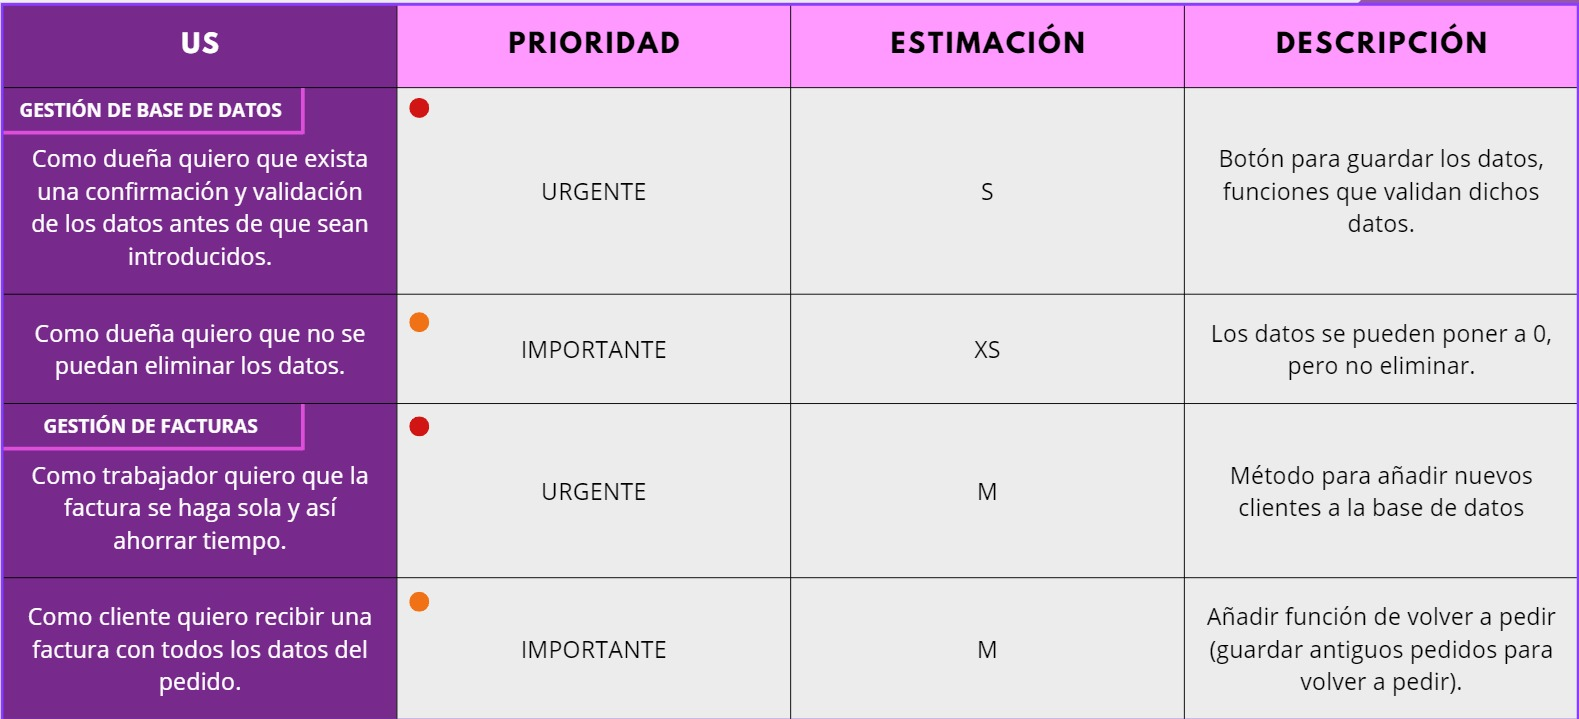
\includegraphics[width=1\textwidth]{figures/backlog-1.jpeg}
    \caption{Caption for backlog-1}
    \label{fig:backlog1}
\end{figure}

\begin{figure}[h]
    \centering
    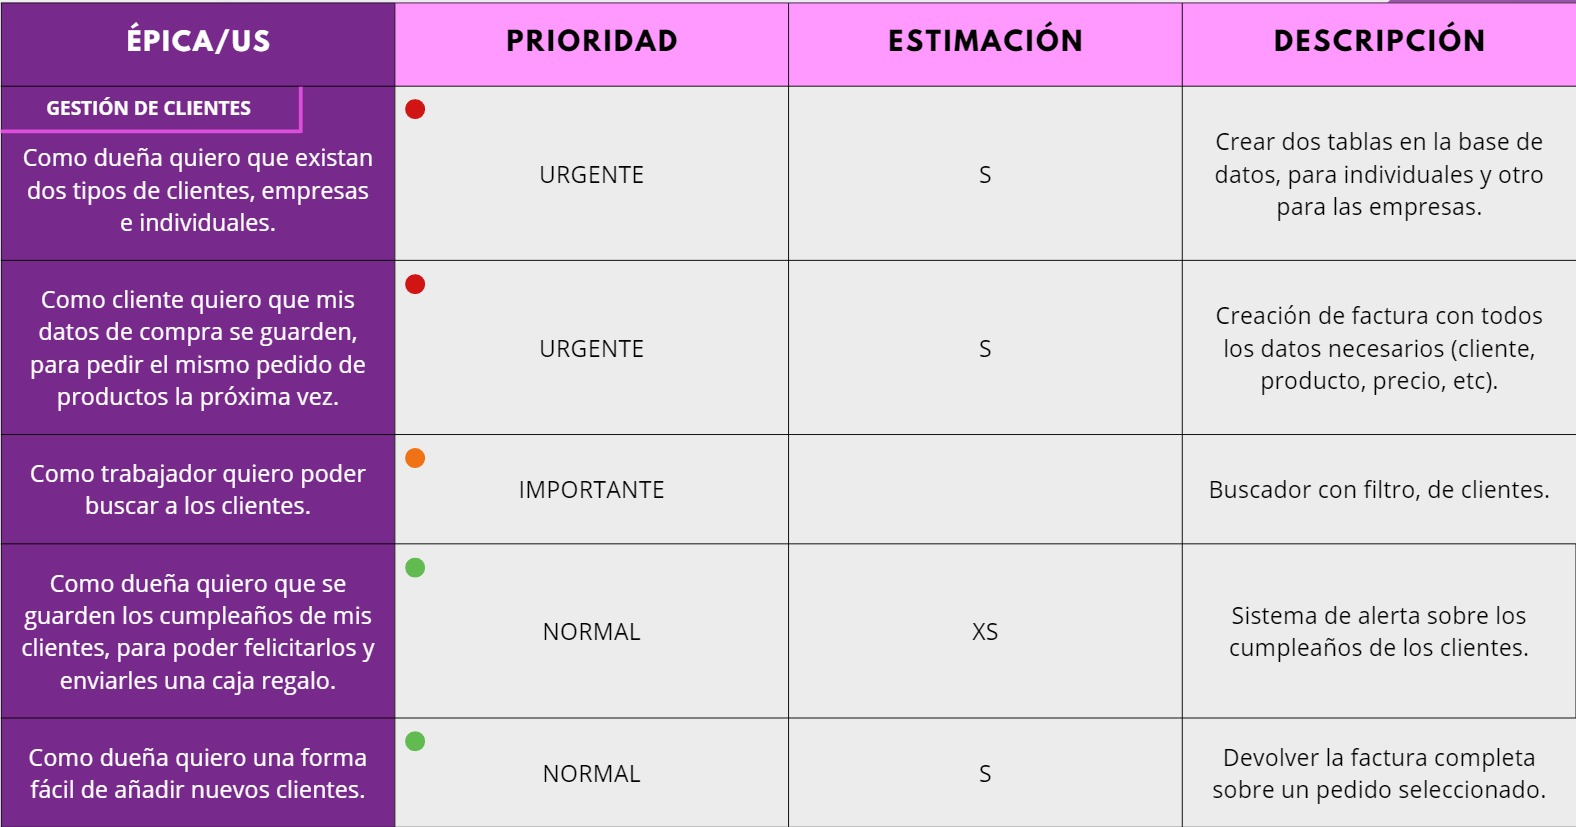
\includegraphics[width=1\textwidth]{figures/backlog-2.jpeg}
    \caption{Caption for backlog-2}
    \label{fig:backlog2}
\end{figure}

\begin{figure}[h]
    \centering
    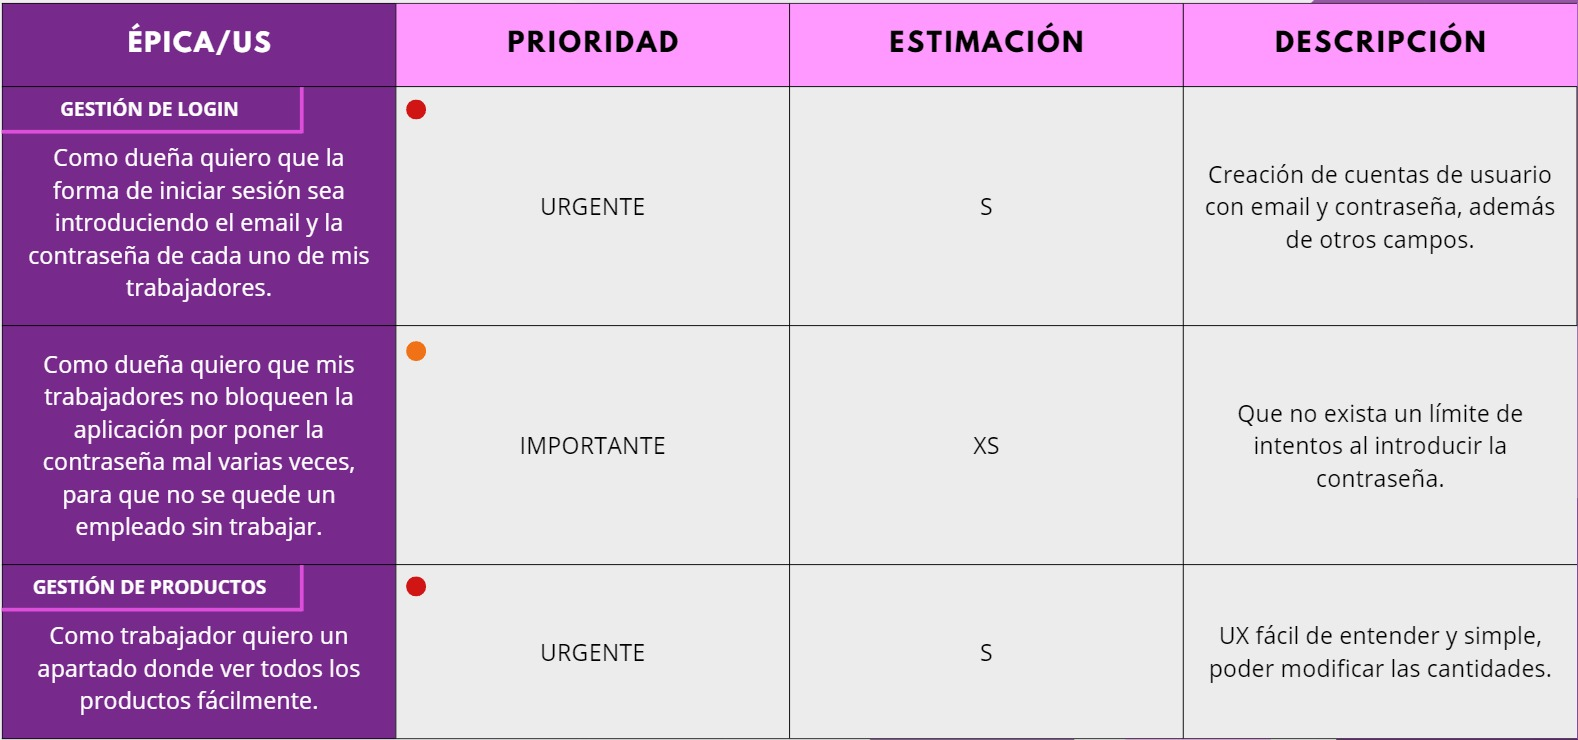
\includegraphics[width=1\textwidth]{figures/backlog-3.jpeg}
    \caption{Caption for backlog-3}
    \label{fig:backlog3}
\end{figure}

\begin{figure}[h]
    \centering
    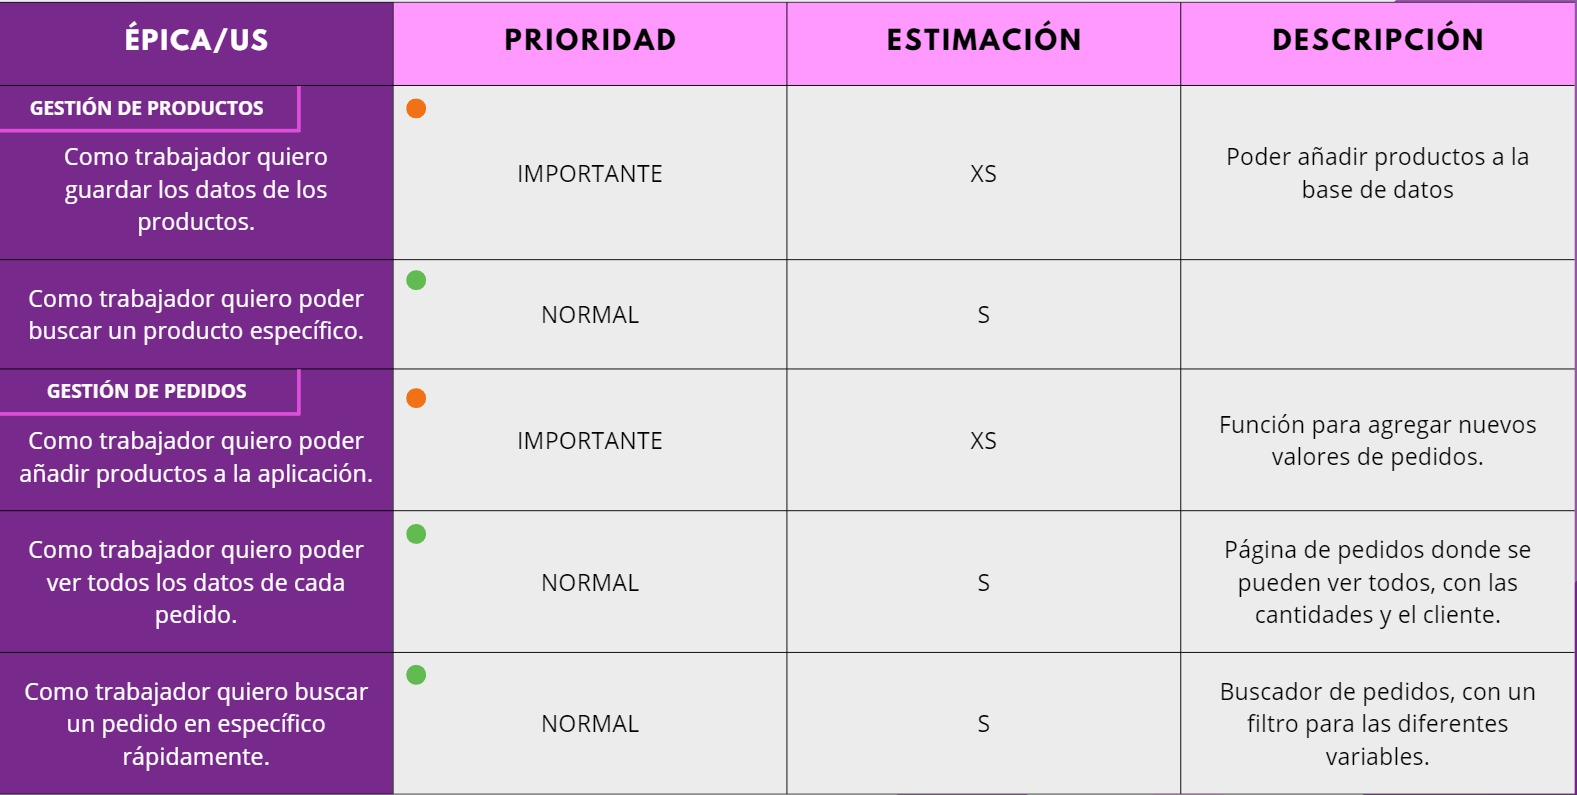
\includegraphics[width=1\textwidth]{figures/backlog-4.jpeg}
    \caption{Caption for backlog-4}
    \label{fig:backlog4}
\end{figure}

\begin{figure}[h]
    \centering
    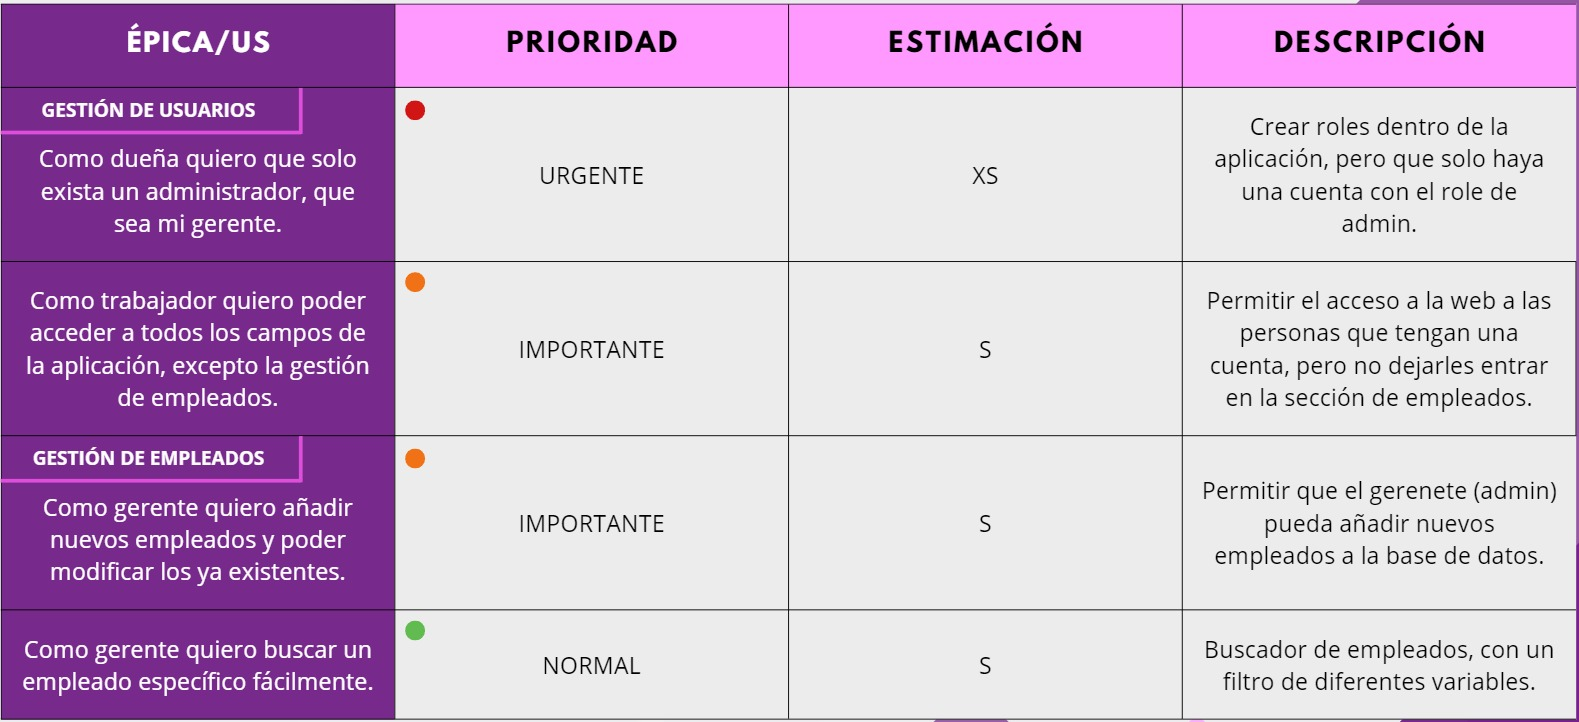
\includegraphics[width=1\textwidth]{figures/backlog-5.jpeg}
    \caption{Caption for backlog-5}
    \label{fig:backlog5}
\end{figure}

\chapter{User Story Mapping}

El mapa de historias de usuarios es una forma muy visual de organizar las historias de usuario y sus tareas relacionadas.

\begin{figure}[h]
    \centering
    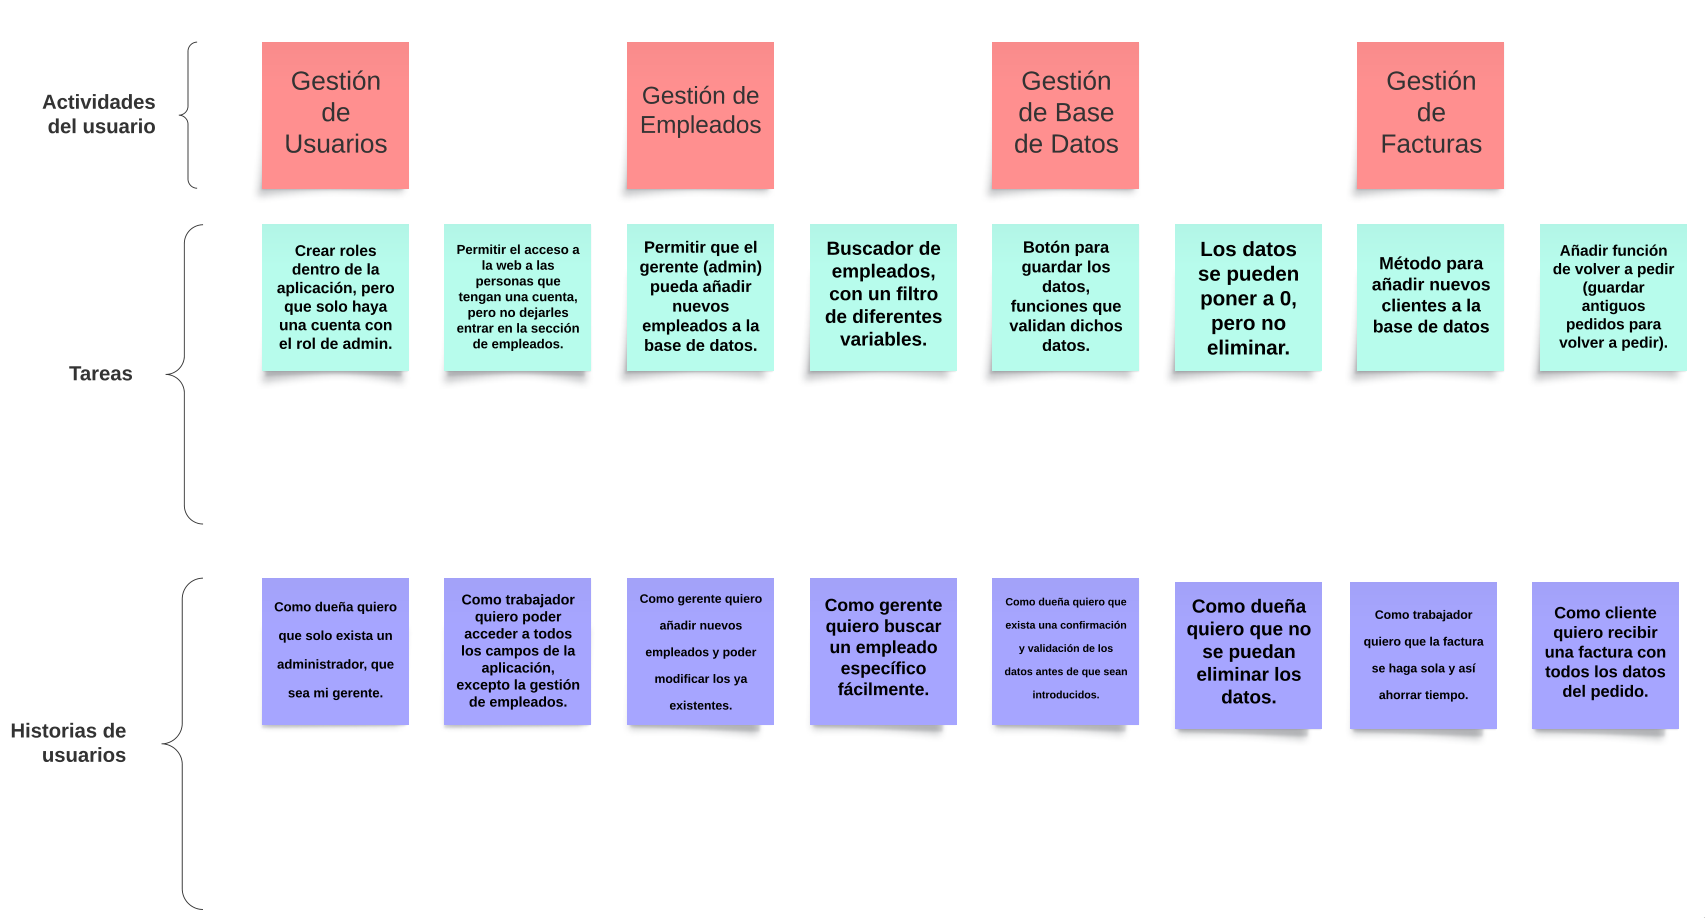
\includegraphics[width=1\textwidth]{figures/mapa-historias-usuarios-1.png}
    \caption{Pimera parte del mapa de las historias de usuario}
    \label{fig:user-story-mapping-1}
\end{figure}

\begin{figure}[h]
    \centering
    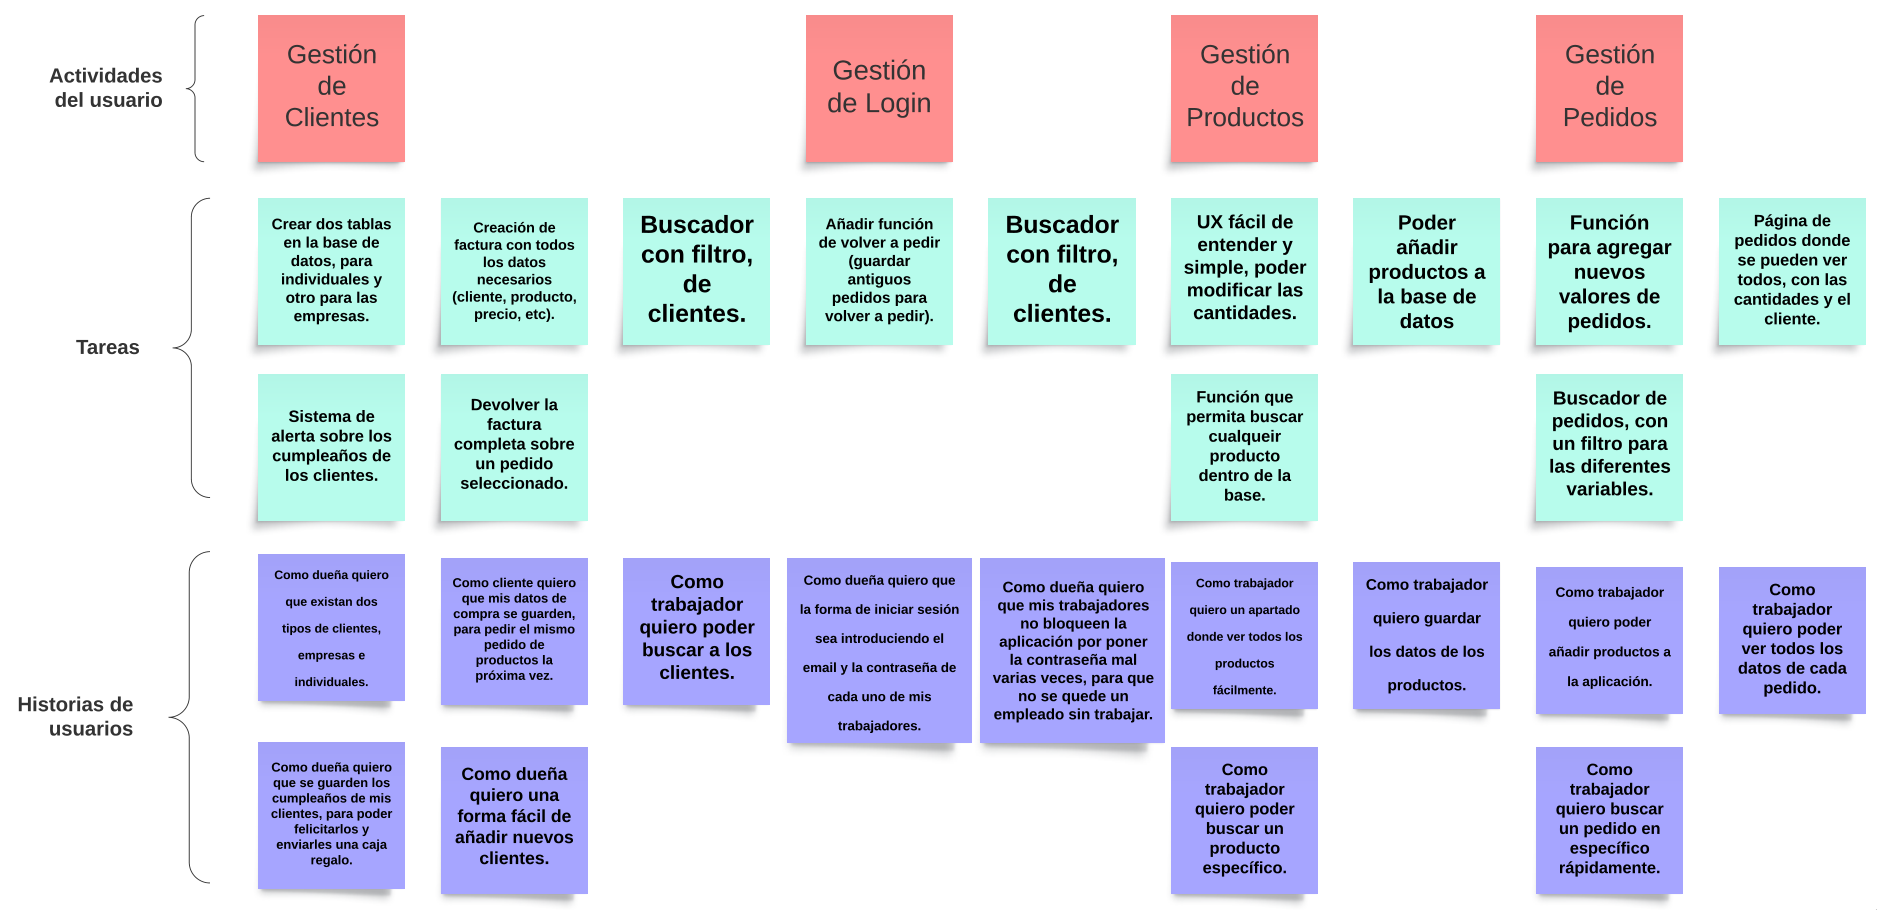
\includegraphics[width=1\textwidth]{figures/mapa-historias-usuarios-2.png}
    \caption{Segunda parte del mapa de las historias de usuario}
    \label{fig:user-story-mapping-2}
\end{figure}

\chapter{Casos de uso}

\begin{figure}[h]
    \centering
    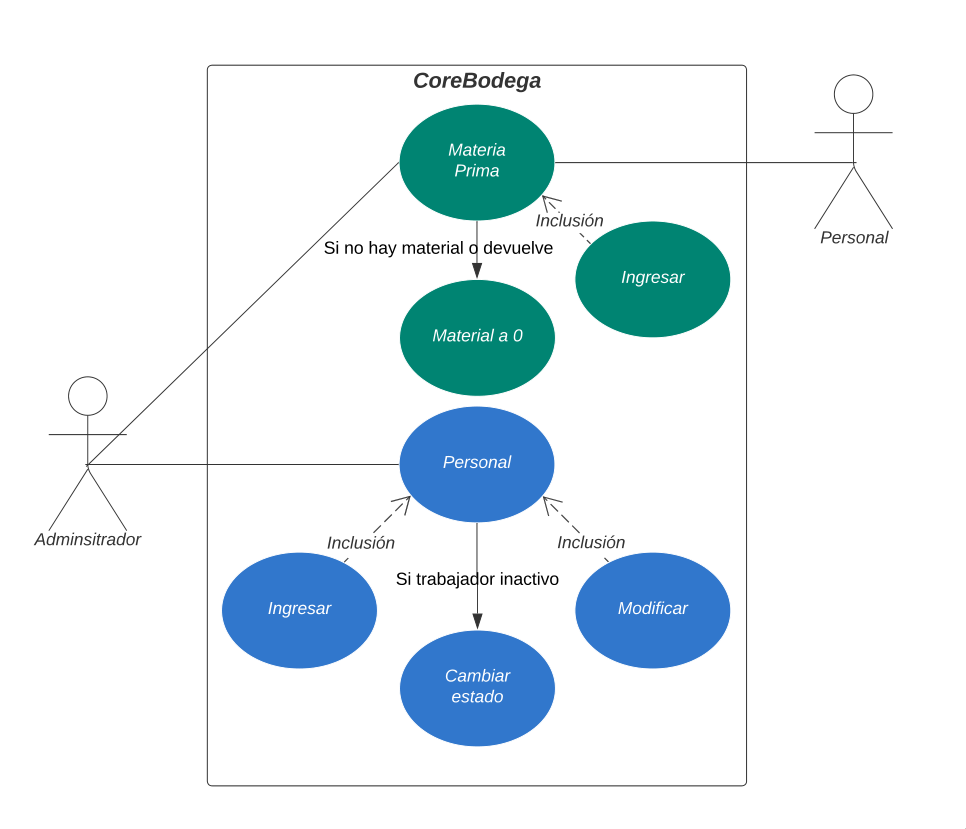
\includegraphics[width=0.9\textwidth]{figures/casos-de-uso-core-bodega.png}
    \caption{Diagrama de casos de uso de CoreBodega}
    \label{fig:corebodega}
\end{figure}

\begin{figure}[h]
    \centering
    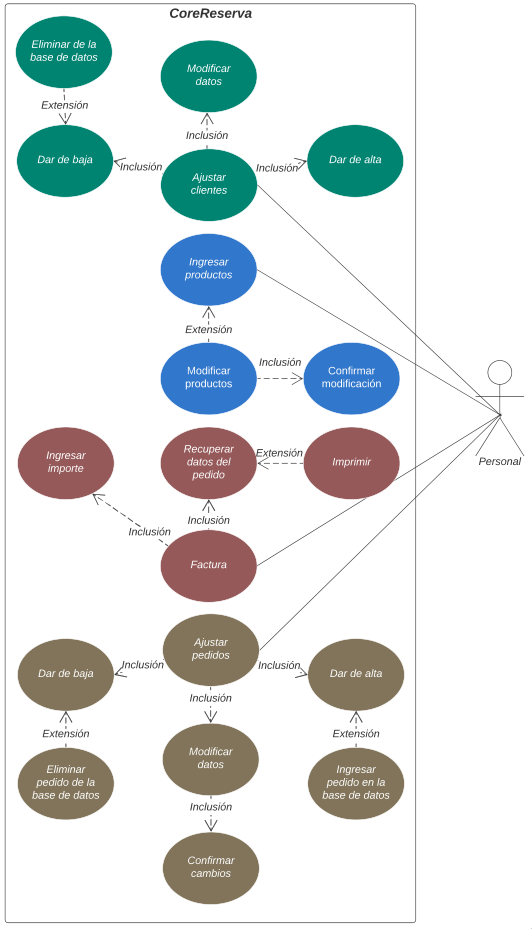
\includegraphics[width=0.8\textwidth]{figures/casos-de-uso-core-reservas.png}
    \caption{Diagrama de casos de uso de CoreReservas}
    \label{fig:corereservas}
\end{figure}

\chapter{Diagrama de clases}

El diagrama de clases nos ayuda a estudiar los diferentes actores de nuestra aplicación.

Con él podremos crear un plan de desarrollo, teniendo en cuenta las dependencias de cada parte del proyecto.

\begin{figure}[h]
    \centering
    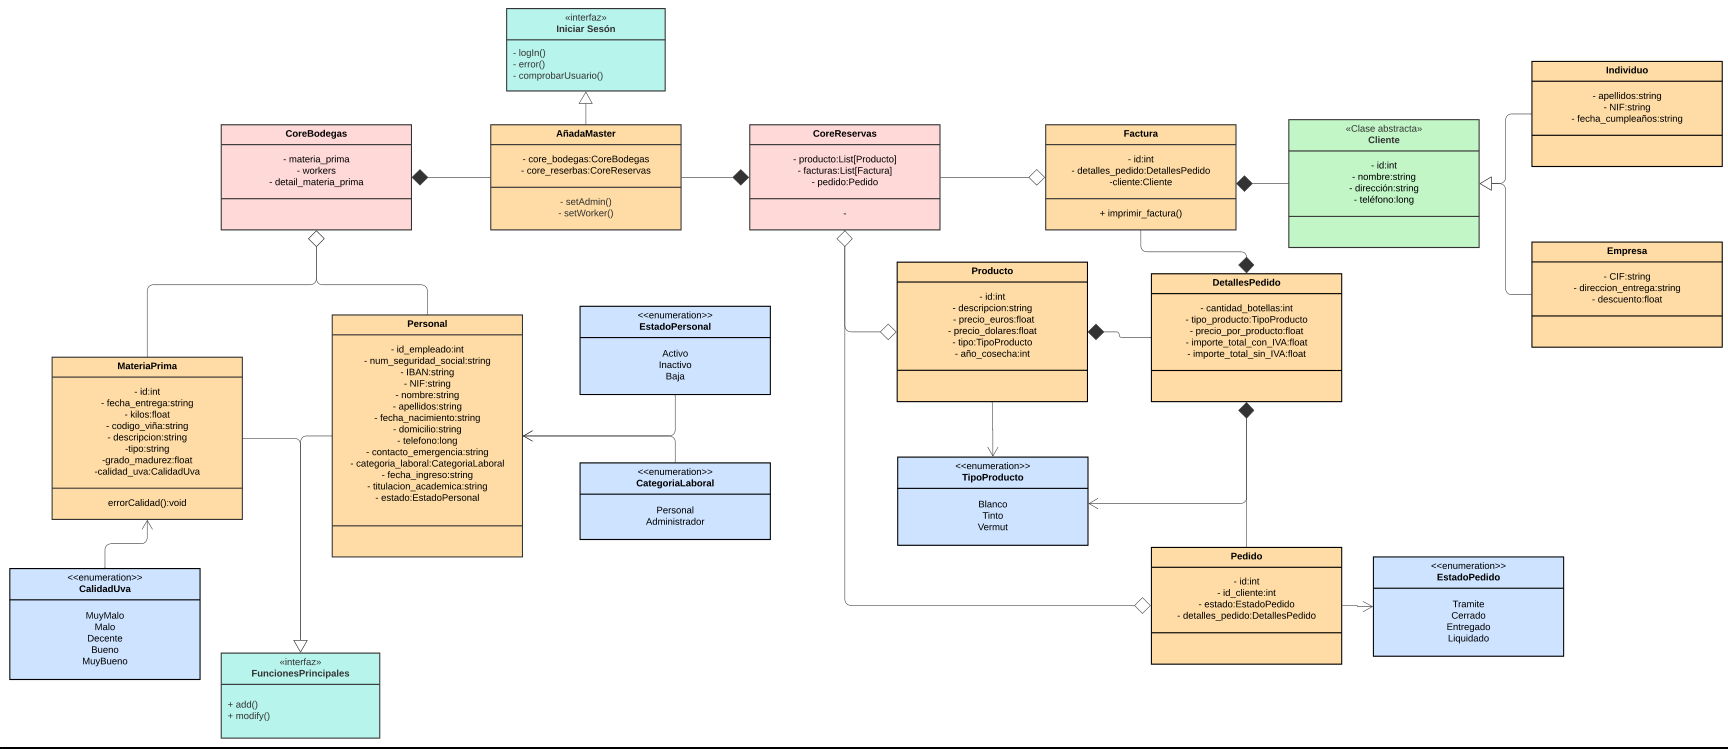
\includegraphics[width=1\textwidth]{figures/diagrama-clases.png}
    \caption{Diagrama de clases UML}
    \label{fig:clases}
\end{figure}

\chapter{Diagramas de secuencia}

\section{Buscar, añadir y modificar elementos}

En este diagrama de secuencia se indica como funcionarían las funciones de buscar, añadir y modificar elementos de la bodega. 

\begin{figure}[h]
    \centering
    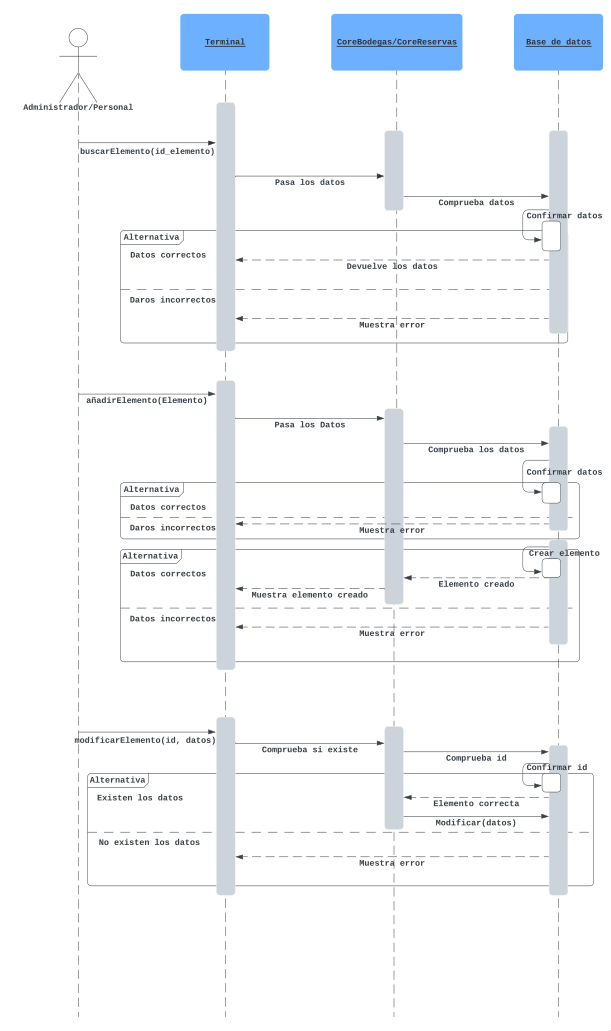
\includegraphics[width=0.4\textwidth]{figures/elementos-secuencia.png}
    \caption{Diagrama de secuencia de elementos}
    \label{fig:elementos}
\end{figure}

\section{Inicio de sesión}

En el segundo diagrama de secuencia veremos como funcionaría el programa de inicio de sesión.

\begin{figure}[h]
    \centering
    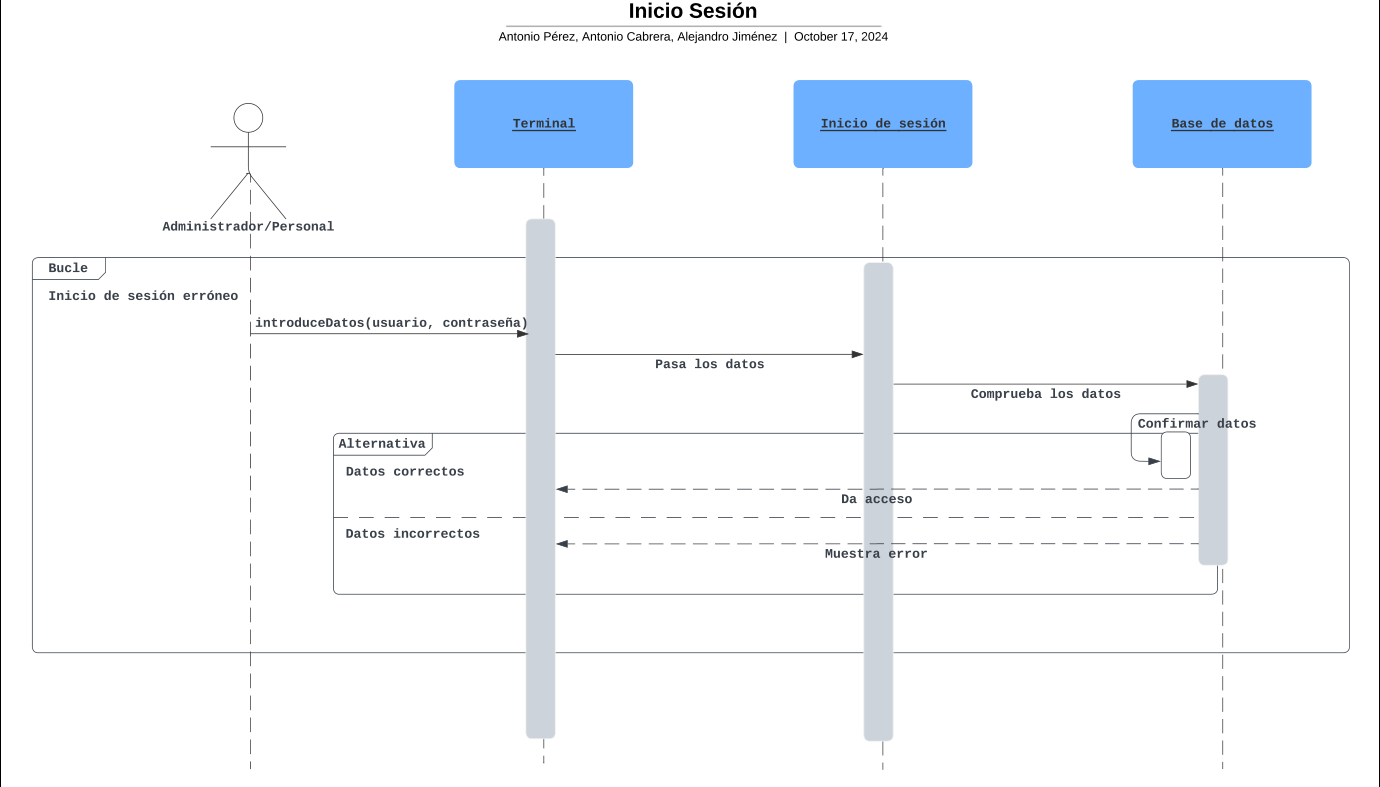
\includegraphics[width=1\textwidth]{figures/inicio-sesion-secuencia.png}
    \caption{Diagrama de secuencia de inicio de sesión}
    \label{fig:login}
\end{figure}

\pagebreak

\section{Personal secuencia}

Por último, en el siguiente diagrama se muestra el funcionamiento de las funciones que tienen que ver con la manipulación del personal.

\begin{figure}[h]
    \centering
    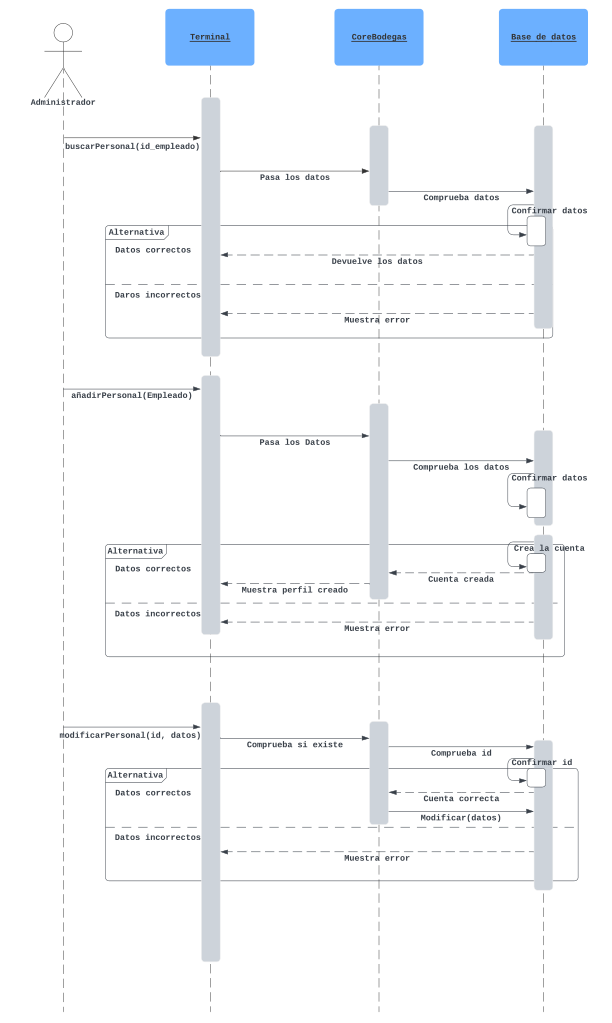
\includegraphics[width=0.5\textwidth]{figures/personal-secuencia.png}
    \caption{Diagrama de secuencia del personal}
    \label{fig:personal}
\end{figure}

\chapter{Diagrama de Gantt}
\newgantttimeslotformat{stardate}{%
\def\decomposestardate##1.##2\relax{%
\def\stardateyear{##1}\def\stardateday{##2}%
}%
\decomposestardate#1\relax%
\pgfcalendardatetojulian{\stardateyear-01-01}{#2}%

\advance#2 by-1\relax%
\advance#2 by\stardateday\relax%
}
\begin{ganttchart}[
hgrid,
vgrid,
expand chart=1.2\textwidth,
time slot format=isodate
]{2024-10-16}{2024-12-18}
    \gantttitlecalendar{month=name, week} \\
    \ganttbar{Task 1}{2024-10-16}{2024-11-02}
\end{ganttchart}



\chapter{Acta de entrevista post mortem}

\textbf{ACTA DE LA ENTREVISTA POST MORTEM REALIZADA POR LOS PARTICIPANTES DE LA EMPRESA K-VATA, PARA REVISAR EL DESARROLLO DEL PROYECTO.}\\

En U-tad, a dieciséis de diciembre de dos mil veinticuatro, siendo las 19:00 horas, se reúnen los siguientes integrantes de la empresa K-VATA para debatir sobre los aspectos realizados durante el desarrollo del proyecto.

\begin{itemize}
    \item Alejandro Jiménez García
    \item Antonio Cabrera Landín
    \item Antonio Pérez Marquéz
\end{itemize}

En la reunión se realizaron las siguientes aportaciones:

\begin{enumerate}
    \item ¿Se ha trabajado correctamente durante todo el proyecto?
    \begin{enumerate}
        \item Antonio Cabrera: Si, en general se ha aplicado una buena metodología de trabajo durante todo el proyecto.
        \item Antonio Pérez: Si, desde un primer momento hemos trabajado en conjunto, discutiendo en grupo cómo hacer las partes del proyecto y que cosas no teníamos claras.
        \item Alejandro Jiménez: Si, desde un principio se decidió que todo se discutía con los demás integrantes para poder aclarar y resolver todos los problemas.
 
    \end{enumerate}
    \item ¿La organización ha estado impuesta desde un principio?
        \begin{enumerate}
            \item Antonio Cabrera: No, al principio estábamos menos organizados, pero a lo largo de las semanas hemos ido mejorando nuestra organización.
            \item Antonio Pérez: No, al comienzo no seguíamos ningún método de organización, no ha sido hasta la última entrega cuando hemos aplicado un buen método de como organizarnos el trabajo.
            \item Alejandro Jiménez: No, nos costó al principio organizarnos fue bastante complicado porque no teníamos claras todas las necesidades del cliente. Pero tras saber todo, nos organizamos y realizamos un buen trabajo.
        \end{enumerate}

    \item ¿Todos los integrantes del proyecto han trabajado adecuadamente?
    \begin{enumerate}
        \item Antonio Cabrera: Si, todos han trabajado adecuadamente.
        \item Antonio Pérez: Si, nos hemos dividido los trabajos de forma equitativa y los tres hemos trabajado una misma cantidad de tiempo, cumpliendo con las fechas y lo que teníamos que entregar.
        \item Alejandro Jiménez: Si, en los trabajos todos los integrantes hemos participado aunque hayan estado “divididos”.
    \end{enumerate}

    \item ¿Se ha entendido desde un principio lo que el cliente nos ha pedido?
    \begin{enumerate}
        \item Antonio Cabrera: No del todo, no fue hasta que tuvimos las reuniones con el cliente que entendimos realmente lo que quería.
        \item Antonio Pérez: Si, desde el principio teníamos la idea correcta de lo que quería el cliente, aunque hubieran ciertas cosas que no estaban explicadas claramente, pero estas dudas las hemos resuelto en las reuniones con el cliente.
        \item Alejandro Jiménez: A medias, desde un principio tuvimos una idea de lo que necesitaba el cliente, pero no fue hasta la primera reunión que aclaramos todas esas dudas y pudimos trabajar al cien por cien.
    \end{enumerate}

    \item ¿Ha existido una buena comunicación entre los integrantes?
    \begin{enumerate}
        \item Antonio Cabrera: Si, la comunicación entre los miembros del equipo ha sido fluida.
        \item Antonio Pérez: Si, hemos comunicado todo lo que había que hacer en cada momento, y se ha transmitido claramente quien se encarga de que parte del trabajo.
        \item Alejandro Jiménez: Si, todos los avances que se han producido durante el desarrollo del trabajo se han ido comunicando, por lo que ha habido una buena comunicación
    \end{enumerate}

    \item ¿Puedes mencionar tres cosas que salieron bien durante este proyecto?
    \begin{enumerate}
        \item Antonio Cabrera: Las entrevistas con el cliente, el ambiente en el equipo y la recogida de requisitos
        \item Antonio Pérez: La comunicación entre los miembros del grupo, el reparto de actividades entre cada miembro del equipo y la preparación a las reuniones con el cliente.
        \item Alejandro Jiménez: La buena relación que hemos tenido, que ha ayudado a que haya una buena comunicación; el desarrollo de los UML, que nos permitieron darle una mayor perspectiva al trabajo; y las presentaciones al cliente, que nos permitieron pulir nuestros errores o cambiarlos totalmente.
    \end{enumerate}

        \item ¿Puedes mencionar tres cosas que no salieron bien durante este proyecto?
        \begin{enumerate}
            \item Antonio Cabrera: Solo puedo encontrar dos cosas que no salieron del todo bien: la primera vez que hicimos las épicas no salieron bien del todo; y la segunda cosa que se puede mejorar es la constancia de trabajo ya que algunas semanas trabajamos mucho y otras menos.
            \item Antonio Pérez: La constancia en el trabajo, algunas semanas trabajamos demasiado en los proyectos de la asignatura, lo que llevó a que las siguientes semanas no tuviéramos tantas ganas de realizar el trabajo; la organización, no nos hemos organizado desde un primer momento; y no comenzar con tiempo el prototipo de la aplicación.
            \item Alejandro Jiménez: Desde un principio no hemos sido constantes, lo que ha generado épocas de gran cantidad de trabajo; la realización de las historias de usuarios, al principio no teníamos claro cómo crearlas pero conseguimos solucionarlo; y el prototipo, nos atrasamos con las demás partes lo que llevó a no terminarlo.
        \end{enumerate}

    \item ¿Tienes alguna sugerencia sobre cómo podemos mejorar para el próximo proyecto?
    \begin{enumerate}
        \item Antonio Cabrera: Podríamos agendar reuniones cada dos días para mantener una constancia adecuada.
        \item Antonio Pérez: Aplicar una metodología ágil desde un primer momento (como la que proponemos nosotros), para organizarnos mejor; y tomar pausas al realizar los trabajos, para no estar quemados en las siguientes tareas.
        \item Alejandro Jiménez: Se podrían aplicar metodologías como SCRUM para poder llevar mejor el proyecto sin que haya grandes acumulaciones de trabajo.
    \end{enumerate}
    
    \item ¿Te gustaría volver a trabajar en un proyecto como este?¿Por qué o por qué no?
    \begin{enumerate}
        \item Antonio Cabrera: Me gustaría más trabajar en un trabajo práctico ya que este era muy teórico.
        \item Antonio Pérez: Si, me gusto mucho el ambiente de trabajo, además, me ha gustado realizar un proyecto desde cero. Y tengo ganas de aplicar desde un primer momento estrategias de trabajo que hemos ido descubriendo.
        \item Alejandro Jiménez: La realización de este proyecto nos ha dado una perspectiva nueva de cómo se realizan los trabajos y no como habíamos hecho con anterioridad, pero me gustaría trabajar más en una parte práctica.
 
    \end{enumerate}

    \item Después de esta experiencia, si pudieras volver a hacer este proyecto, ¿qué harías de
    forma diferente?
    \begin{enumerate}
        \item Antonio Cabrera: Intentaría hacer una prueba de concepto del proyecto funcionando de verdad.
        \item Antonio Pérez: Empezaría con el desarrollo del prototipo mucho antes, en vez de esperar a que el resto de apartados estén bien pulidos, de esta forma podríamos tener un feedback del cliente a medida que avanzamos con la aplicación.
        \item Alejandro Jiménez: Desde un principio realizaría una agenda para no acumular trabajo. 
    \end{enumerate}
\end{enumerate}




\end{document}
